\newif\ifIEEEavailable
\IfFileExists{IEEEtran.cls}{\IEEEavailabletrue}{\IEEEavailablefalse}
\ifIEEEavailable
  \documentclass[conference]{IEEEtran}
\else
  \documentclass[10pt,twocolumn]{article}
  \newenvironment{IEEEkeywords}{\par\small\noindent\textbf{Index Terms---}}{\par}
\fi

\usepackage{amsmath,amssymb,booktabs,graphicx,multirow}
\usepackage[hidelinks]{hyperref}
\graphicspath{{results/figures/}{../results/figures/}}

\newcommand{\vect}[1]{\boldsymbol{#1}}
\newcommand{\R}{\mathbb{R}}
\newcommand{\tr}{\operatorname{tr}}
\newcommand{\Local}{\textsc{Local}}
\newcommand{\FedTwenty}{\textsc{Fed20}}

\title{Federated Personalized LPV Identification for Cold-Start Control in Heterogeneous Vehicle Fleets}

\ifIEEEavailable
  \author{\IEEEauthorblockN{Jakob Weber et al.}
  \IEEEauthorblockA{Author affiliations to be completed before submission}}
\else
  \author{Jakob Weber et al.\\\small Author affiliations to be completed before submission}
\fi

\begin{document}
\maketitle

\begin{abstract}
A newly deployed vehicle may not yet have sufficiently informative data to
identify an individualized controller, whereas previously observed fleet
clients collectively cover a broader range of dynamics and operating
conditions. A single global model cannot exploit this information without
suppressing control-relevant heterogeneity. This paper proposes a personalized
federated framework for cold-start linear-parameter-varying (LPV)
identification. Each fleet client estimates three structured log-parameters and
a local uncertainty approximation. Additive sufficient statistics then learn a
heteroscedastic mixture with an unknown number of latent groups and construct a
controller-gain-aware low-rank backbone for each group. A new client selects a
backbone and estimates one client-specific coordinate from a short local
record; its trajectory and coordinate remain local. The identified model is
used to synthesize a speed-scheduled controller and evaluated on nonlinear,
heterogeneous bicycle plants. In a frozen ten-fleet confirmation, the method
with 20\% rotating participation reduces aggregate yaw-rate tracking RMSE by
17.27\% relative to independent local identification at a 0.75~s calibration
budget, with nine of ten fleet-wise wins and complete empirical feasibility. A
paired retrospective analysis estimates a 16.90\% mean improvement with a 95\%
fleet-bootstrap interval of 11.79--21.10\%. The advantage contracts to parity
as local information increases, while a fixed narrow participant subset
exposes a coverage failure. Federated LPV learning is therefore most useful as
a fleet-informed cold-start prior, not as a universal replacement for
well-excited local identification.
\end{abstract}

\begin{IEEEkeywords}
federated learning, linear parameter-varying systems, system identification,
personalized learning, vehicle control
\end{IEEEkeywords}

\section{Introduction}
\label{sec:introduction}

Model-based vehicle controllers must accommodate two different forms of
variation. First, the dynamics change with measurable operating conditions,
such as longitudinal speed. Linear-parameter-varying (LPV) models expose this
dependence to controller synthesis instead of absorbing it into model error.
Second, vehicles retain persistent differences caused by mass, inertia, tire
properties, and configuration. These differences remain even at the same
operating point. A useful fleet model must therefore represent both scheduling
and structural heterogeneity.

Independent system identification is a natural solution when every vehicle
has sufficiently rich data. In the present structured setting it is also a
strong baseline: only three physically meaningful ratios must be estimated,
and local identification approaches the individual optimum once excitation is
adequate. The difficult case occurs earlier. A newly deployed vehicle may have
only a short and incompletely exciting record, precisely when its first
controller must be calibrated. Requiring a complete local experiment for every
new client repeats effort and ignores information already accumulated across
the fleet.

Straightforward fleet sharing does not resolve the problem. One global model
reduces variance but biases structurally different vehicles toward the same
dynamics. A separate model for every vehicle preserves individuality but offers
no transfer. Family-pooled models occupy a useful middle ground, yet require
compatibility labels to be known in advance and cannot represent variation
within a family. The missing capability is to discover reusable fleet
structure, transfer it to an unseen vehicle, and retain a small local degree of
freedom for personalization.

We address this gap with a federated latent-backbone method for structured LPV
identification. Previously observed clients estimate local physical summaries
and their Gauss--Newton uncertainty approximations. An iterative server learns
a heteroscedastic latent mixture from additive sufficient statistics and
selects its order by the Bayesian information criterion (BIC). Within each
learned group, a metric derived from scheduled-controller gain sensitivities
defines a low-dimensional affine backbone. A new client downloads the
backbones, selects a compatible group, and estimates a single coordinate using
its short record. Raw trajectories and new-client coordinates are not shared.

The resulting interpretation is deliberately narrower than generic claims that
federation should always outperform local estimation. Fleet knowledge acts as
a control-relevant prior while the new client is information limited. As more
local excitation becomes available, the client first adapts within a
fleet-supported direction and eventually reaches local parity. The shared
representation is useful only if participation covers the fleet dynamics;
participation rate alone is not an adequate reliability measure.

The paper makes four contributions:
\begin{enumerate}
  \item a personalized LPV architecture that separates measured operating
  variation, latent fleet heterogeneity, and residual client individuality;
  \item an unknown-order federated heteroscedastic-mixture algorithm based on
  additive statistics, followed by controller-gain-aware low-rank backbone
  construction;
  \item a frozen nonlinear closed-loop confirmation showing a 17.27\% reduction
  in cold-start tracking error with 20\% rotating participation; and
  \item a mechanism and participation audit showing when the group prior, local
  coordinate, and cumulative fleet coverage create---or destroy---the benefit.
\end{enumerate}

The contribution differs from our preceding uncertainty-aware clustered
identification study, which focused on recovering compatible regimes for
controller design. Here, clustering is not the endpoint: explicit LPV
scheduling, an unknown-order federated representation, and local adaptation of
an unseen client form the central transfer mechanism.

\section{Related Work and Positioning}
\label{sec:related}

Federated learning enables clients to optimize a shared model without moving
their raw records to a central database \cite{mcmahan2017fedavg}. Heterogeneous
client populations have motivated clustered and personalized variants that
learn several shared models or decompose a model into shared and local parts
\cite{smith2017mocha,fallah2020personalized}. Most such methods are developed
for prediction losses and high-dimensional statistical models. Their direct
use for control is complicated because parameter error, model error, and
closed-loop performance need not rank candidate representations identically.

Federated system identification has consequently begun to combine local
estimators with physically structured aggregation. Our earlier method used
local recursive estimates, covariance-aware clustering, and group-level
controller design \cite{weber2026ifac}. The present work retains uncertainty as
an input to grouping but changes the scientific question from regime recovery
to cold-start transfer. It uses batch output-error identification of an LPV
parameterization, learns the number of groups, constructs control-aware
low-rank backbones, and evaluates local adaptation by a previously unseen
client.

LPV modeling and gain scheduling provide established tools for systems whose
dynamics depend on measurable operating variables \cite{toth2010lpv}. In the
vehicle setting, the same scheduling variable should not be expected to explain
persistent variation in inertial and tire parameters. Our earlier regime-map
experiments confirm this distinction within the tested benchmark: scheduling
addresses broad speed variation, whereas specialization addresses structural
separation. This motivates the explicit three-level decomposition used below.

\section{Problem Formulation}
\label{sec:problem}

\subsection{Fleet and cold-start setting}

Let $\mathcal I=\{1,\ldots,N\}$ denote previously observed fleet clients. Client
$i$ retains a local record
\begin{equation}
  \mathcal D_i=\{\vect y_{i,t},\delta_{i,t},v_{i,t}\}_{t=1}^{T_i},
\end{equation}
containing measured lateral states or outputs $\vect y_{i,t}$, steering input
$\delta_{i,t}$, and longitudinal speed $v_{i,t}$. A separate, unseen client
$j$ has only a short calibration record $\mathcal D_j^{(\tau)}$ of duration
$\tau$. The goal is to design a speed-scheduled controller for client $j$ using
its short local record and a representation learned from $\mathcal I$, without
uploading either client's raw trajectory.

This is an asymmetric transfer setting. The fleet representation is learned
once from broader historical coverage, whereas the new-client comparison asks
how much local calibration is required at deployment. It is not an equal-total-
data comparison between federation and local identification.

\subsection{Nonlinear plant and structured LPV model}

Evaluation uses a planar bicycle model with lateral velocity $v_y$, yaw rate
$r$, steering angle $\delta$, longitudinal speed $v_x$, and nonlinear saturated
tire forces. For controller synthesis, the client fits a structured LPV
approximation whose scheduling variable is $v_x$. The identifiable positive
ratios are
\begin{equation}
 \vect p_i=
 \begin{bmatrix}C_{f,i}/m_i\\ C_{r,i}/m_i\\ m_i/I_{z,i}\end{bmatrix},
 \qquad \vect z_i=\log \vect p_i\in\R^3,
 \label{eq:ratios}
\end{equation}
where $C_f,C_r$ are axle cornering stiffnesses, $m$ is mass, and $I_z$ is yaw
inertia. At a fixed speed the approximation is linear in the lateral states;
across speed it defines the LPV matrices
\begin{equation}
 \dot{\vect x}=A(\rho;\vect p_i)\vect x+B(\rho;\vect p_i)\delta,
 \qquad \rho=v_x.
 \label{eq:lpv}
\end{equation}
The logarithm enforces positivity and makes multiplicative physical variation
approximately additive.

Client $i$ obtains
\begin{equation}
 \widehat{\vect z}_i=\arg\min_{\vect z\in\mathcal Z}
 L_i(\vect z;\mathcal D_i),
 \label{eq:localoe}
\end{equation}
where $L_i$ is the batch output-error loss and $\mathcal Z$ is a public physical
box. A Gauss--Newton approximation $C_i$ describes local estimation uncertainty.
It is used as a heteroscedastic measurement covariance, not interpreted as an
exact posterior.

\subsection{Control objective}

Each estimated parameter vector is mapped to scheduled feedback and prefilter
gains over a fixed speed grid. Nonlinear evaluation uses yaw-rate tracking RMSE
\begin{equation}
 e_{j,s}=\sqrt{\frac{1}{T_s}\sum_{t=1}^{T_s}
 \bigl(r_{j,s,t}-r_{s,t}^{\mathrm{ref}}\bigr)^2},
 \label{eq:tracking}
\end{equation}
for new client $j$ and scenario $s$. Empirical feasibility additionally
requires finite simulation and compliance with steering and lateral-
acceleration limits. These tests and frozen-point spectral radii are diagnostics;
they do not constitute a nonlinear time-varying stability proof.

\section{Federated Latent-Backbone Method}
\label{sec:method}

\subsection{Uncertainty-aware latent groups}

The fleet summaries are modeled by a heteroscedastic Gaussian mixture
\begin{equation}
 \widehat{\vect z}_i\sim
 \sum_{g=1}^{K}\pi_g\,
 \mathcal N\!\left(\vect\mu_g,C_i+S_g\right),
 \label{eq:mixture}
\end{equation}
where $\vect\mu_g$ is a group center and $S_g$ captures physical variation not
explained by $C_i$. For a current server state
$\Theta=\{\pi_g,\vect\mu_g,S_g\}_{g=1}^{K}$, client $i$ evaluates
\begin{equation}
 q_{ig}=\frac{\pi_g\mathcal N(\widehat{\vect z}_i;
 \vect\mu_g,C_i+S_g)}{\sum_h\pi_h\mathcal N(\widehat{\vect z}_i;
 \vect\mu_h,C_i+S_h)}.
 \label{eq:responsibility}
\end{equation}

The client then contributes, for each group, responsibility mass, precision,
information vector, and uncertainty-corrected scatter. Denoting
$P_{ig}=(C_i+S_g)^{-1}$, representative additive quantities are
\begin{align}
 n_g &= \sum_i q_{ig}, \qquad
 \Lambda_g = \sum_i q_{ig}P_{ig},\nonumber\\
 \vect h_g &= \sum_i q_{ig}P_{ig}\widehat{\vect z}_i,\nonumber\\
 Q_g &= \sum_i q_{ig}
 (\widehat{\vect z}_i-\vect\mu_g)(\widehat{\vect z}_i-\vect\mu_g)^\top.
 \label{eq:suffstats}
\end{align}
Only cohort sums of these terms are required by the server. It updates the
mixture state with fixed damping and broadcasts the new state for the next
round. Candidate orders $K\in\{1,\ldots,6\}$ are fitted separately. Clients
finally contribute local likelihood and responsibility masses, enabling a BIC
comparison subject to a minimum effective group size.

\subsection{Control-aware group backbone}

After selecting $K$, hard group assignments provide additive group counts,
first moments, and symmetric second moments. For each group, the server forms a
metric from finite-difference sensitivities of the scheduled controller gain
table $\mathcal K(\vect z)$,
\begin{equation}
 W_g=J_{K,g}^{\top}J_{K,g}+\eta I,
 \qquad
 J_{K,g}=\left.\frac{\partial\operatorname{vec}\mathcal K(\vect z)}
 {\partial\vect z}\right|_{\vect z=\vect\mu_g},
 \label{eq:gainmetric}
\end{equation}
with small $\eta>0$. Weighted principal-component analysis of the aggregated
group covariance yields a direction $U_g$ and the affine representation
\begin{equation}
 \vect z\approx\vect\mu_g+U_g\vect a.
 \label{eq:backbone}
\end{equation}
The metric makes the basis sensitive to scheduled gains; it is not claimed to
optimize nonlinear tracking loss directly.

\subsection{New-client adaptation}

The unseen client receives $\{\vect\mu_g,U_g\}_{g=1}^{K}$ and, for each group,
solves
\begin{equation}
 \widehat{\vect a}_{jg}=\arg\min_{\vect a}
 L_j(\vect\mu_g+U_g\vect a;\mathcal D_j^{(\tau)})
 +\lambda\|\vect a\|_2^2.
 \label{eq:personalization}
\end{equation}
It selects the group with the lowest local criterion and synthesizes its
controller from $\widehat{\vect z}_j=\vect\mu_g+U_g\widehat{\vect a}_{jg}$.
Rank zero corresponds to the learned center; rank one provides one continuous
client-specific coordinate. The group decision, coordinate, and calibration
record remain local.

\begin{table}[t]
\centering
\caption{Information and trust boundary of the evaluated protocol.}
\label{tab:trust}
\small
\begin{tabular}{p{0.34\columnwidth}p{0.55\columnwidth}}
\toprule
Quantity & Visibility\\
\midrule
Raw trajectories & retained by each client\\
Local estimate and covariance & local input to message computation\\
Additive statistics & cohort sums received by server\\
Mixture and backbones & server model, broadcast to clients\\
New-client group and coordinate & retained by new client\\
True generating family & evaluation only\\
\bottomrule
\end{tabular}
\end{table}

\subsection{Federated protocol and communication}

Algorithmically, initialization uses additive counts, first moments, and
second moments. Each of 30 mixture rounds consists of a server broadcast,
local responsibility evaluation, and aggregation of the statistics in
\eqref{eq:suffstats}. Model-order selection adds responsibility masses and one
likelihood scalar per candidate, after which final moments determine the
backbones. Thus the approach is federated sufficient-statistic estimation, not
federated averaging.

The implementation emulates clients and server in one process. Its messages
are compatible with additive secure aggregation, but no cryptographic protocol
or differential privacy is implemented. Communication counts independent
float32 payload scalars and excludes headers, cryptographic expansion,
retransmissions, and the one-time new-client download. We distinguish complete
unknown-$K$ discovery from a fixed-$K$ update in which the selected order is
reused.

\section{Experimental Design}
\label{sec:experiments}

\subsection{Fleet generation and data}

Each fleet contains 180 representation-learning clients drawn from three
synthetic physical populations, with 60 clients per population, and 30 separate
new clients used only for evaluation. Fleet clients provide 4.75~s of
complementary calibration data spanning speeds from 10 to 30~m/s. New clients
receive either 0.75 or 1.25~s of local data. The server considers one through
six mixture components, requires an effective group size of at least ten, and
uses 30 communication rounds with damping 0.35.

Controllers are evaluated on three unseen varying-speed or constant-speed
nonlinear scenarios. The main confirmation uses ten reserved fleet seeds that
were not inspected during method development. Client/scenario outcomes are
averaged within a fleet; the fleet seed is the independent statistical unit.
All primary tracking values are reported in rad/s.

\subsection{Compared methods}

\begin{table}[t]
\centering
\caption{Methods in the matched confirmation-fleet analysis.}
\label{tab:methods}
\small
\begin{tabular}{lp{0.61\columnwidth}}
\toprule
Method & Shared and local information\\
\midrule
\Local & three parameters fitted from new-client data\\
GlobalK1 & one fleet-wide center; no local coordinate\\
LearnedCenter & learned group center; no coordinate\\
CentralRank1 & centralized summaries; one local coordinate\\
\FedTwenty Rank1 & 20\% rotating federation; one coordinate\\
ExactIndividual & true individual parameters; diagnostic only\\
\bottomrule
\end{tabular}
\end{table}

The frozen confirmation additionally includes 100\% and 50\% participation.
Fed20, Fed50, and Fed100 sample clients independently in every round. A separate
development stress test evaluates uniform rotating participation, a fixed
20\% subset, family- and operating-point-biased availability, and 50\% message
dropout after uniform selection.

\subsection{Metrics and statistical analysis}

The primary metric is nonlinear yaw-rate RMSE from \eqref{eq:tracking}.
Secondary metrics are the Euclidean norm of log-parameter error, relative
Frobenius error of scheduled gain tables, empirical feasibility, learned group
count, adjusted Rand index (ARI), cumulative client coverage, and payload.
ARI uses synthetic generating labels for evaluation only.

The frozen confirmation reports the ratio of aggregate fleet means. A
retrospective mechanism analysis computes paired percentage improvements within
each of the ten fleets and resamples those fleet effects 50,000 times. Its 95\%
percentile intervals quantify consistency but are not a second blind
confirmation. The two percentage estimands are therefore labeled separately.

\section{Results}
\label{sec:results}

\subsection{Cold-start benefit under partial participation}

Table~\ref{tab:confirmation} gives the frozen confirmation. With 0.75~s of
new-client data, every shared heterogeneous representation improves upon
\Local. \FedTwenty achieves 0.010518~rad/s compared with 0.012714~rad/s for
\Local, corresponding to a 17.27\% reduction by the preregistered ratio-of-
aggregate-means convention. It remains close to the centralized and full-
participation counterparts despite using only 20\% of clients per round. All
evaluated controllers satisfy the empirical feasibility criteria.

\begin{table}[t]
\centering
\caption{Frozen confirmation: nonlinear tracking RMSE [rad/s]. ``vs. Local''
is the ratio of aggregate means; negative values are improvements.}
\label{tab:confirmation}
\small
\setlength{\tabcolsep}{3pt}
\begin{tabular}{lrrrr}
\toprule
& \multicolumn{2}{c}{0.75~s} & \multicolumn{2}{c}{1.25~s}\\
Method & RMSE & vs. Local & RMSE & vs. Local\\
\midrule
Local   & 0.012714 & 0.00\%  & 0.007557 & 0.00\%\\
Central & 0.010731 & $-15.59$\% & 0.007530 & $-0.36$\%\\
Fed100  & 0.010762 & $-15.35$\% & 0.007531 & $-0.34$\%\\
Fed50   & 0.010648 & $-16.24$\% & 0.007539 & $-0.24$\%\\
Fed20   & 0.010518 & $-17.27$\% & 0.007562 & $+0.07$\%\\
\bottomrule
\end{tabular}
\end{table}

At 1.25~s, the methods converge: the frozen progressive Fed20 policy is only
0.07\% worse than Local. This contraction is central to the interpretation.
Federation regularizes an information-limited estimate; it does not replace a
well-informed local fit. The full-participation method is control-equivalent to
Central within 0.3\%, although it misses the deliberately strict 0.1\%
equivalence gate and is not described as numerically identical.

\begin{figure}[t]
\centering
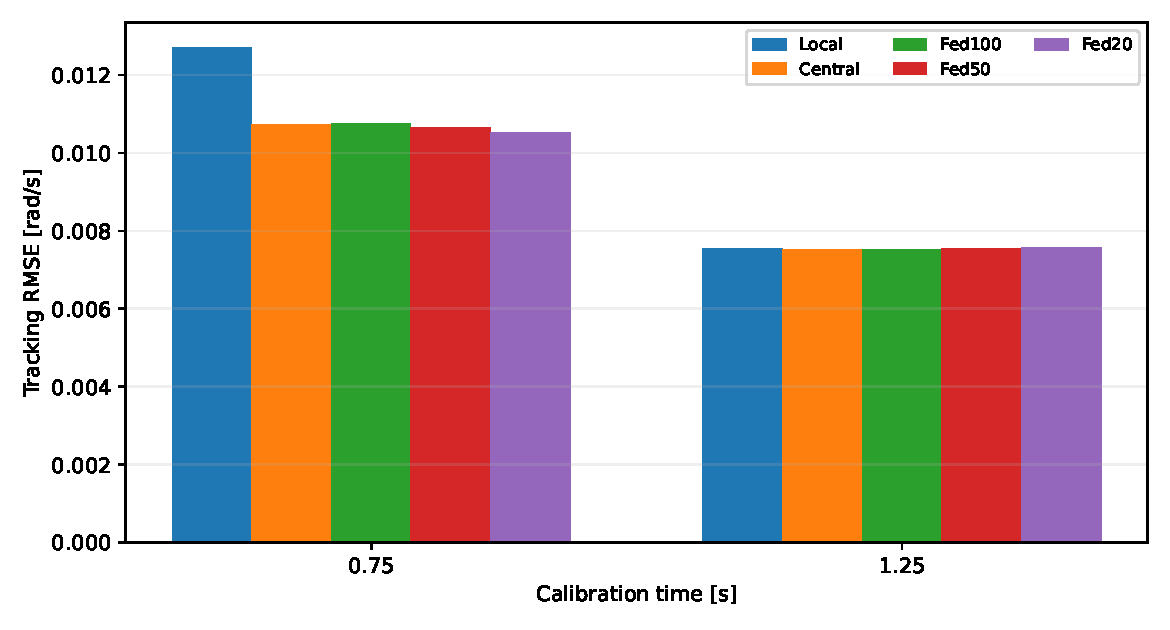
\includegraphics[width=\linewidth]{experiment_9k_blind_confirmation.pdf}
\caption{Blind confirmation of the shared-backbone method. The fleet-informed
advantage is concentrated at the shorter calibration budget.}
\label{fig:confirmation}
\end{figure}

\subsection{What produces the improvement?}

The matched retrospective ablation in Table~\ref{tab:ablation} separates a
global center, latent group structure, and continuous personalization. At
0.75~s, GlobalK1 improves over Local by a paired mean of 8.43\%, but wins only
six fleets. LearnedCenter improves Local by 14.47\%, wins all ten fleets, and
has a 95\% interval of 9.73--19.48\%. The group structure therefore explains
most of the robust cold-start gain.

\begin{table}[t]
\centering
\caption{Matched mechanism analysis on confirmation fleets. Intervals resample
paired fleet-wise percentage improvements.}
\label{tab:ablation}
\scriptsize
\setlength{\tabcolsep}{3pt}
\begin{tabular}{llrr}
\toprule
Budget & Comparison & Mean [\%] & 95\% CI [\%]\\
\midrule
0.75 s & Fed20R1--Local & 16.90 & [11.79, 21.10]\\
0.75 s & Center--Local & 14.47 & [9.73, 19.48]\\
0.75 s & GlobalK1--Local & 8.43 & [2.50, 14.57]\\
0.75 s & Center--GlobalK1 & 5.95 & [$-0.44$, 11.66]\\
0.75 s & Fed20R1--Center & 2.20 & [$-4.56$, 8.79]\\
1.25 s & Fed20R1--Center & 4.21 & [2.40, 6.36]\\
\bottomrule
\end{tabular}
\end{table}

The rank-one coordinate adds 2.20\% over LearnedCenter at 0.75~s, but its
interval crosses zero. It would therefore be incorrect to attribute the entire
cold-start improvement to continuous personalization. At 1.25~s, the role
changes: rank one improves LearnedCenter by 4.21\%, with ten of ten wins and an
interval of 2.40--6.36\%. The emerging mechanism is staged. A discrete group
prior is most valuable under severe information scarcity; a local coordinate
becomes estimable as additional excitation arrives. Rank two is unnecessary in
the matched analysis and overfits at the shorter budget.

\begin{figure}[t]
\centering
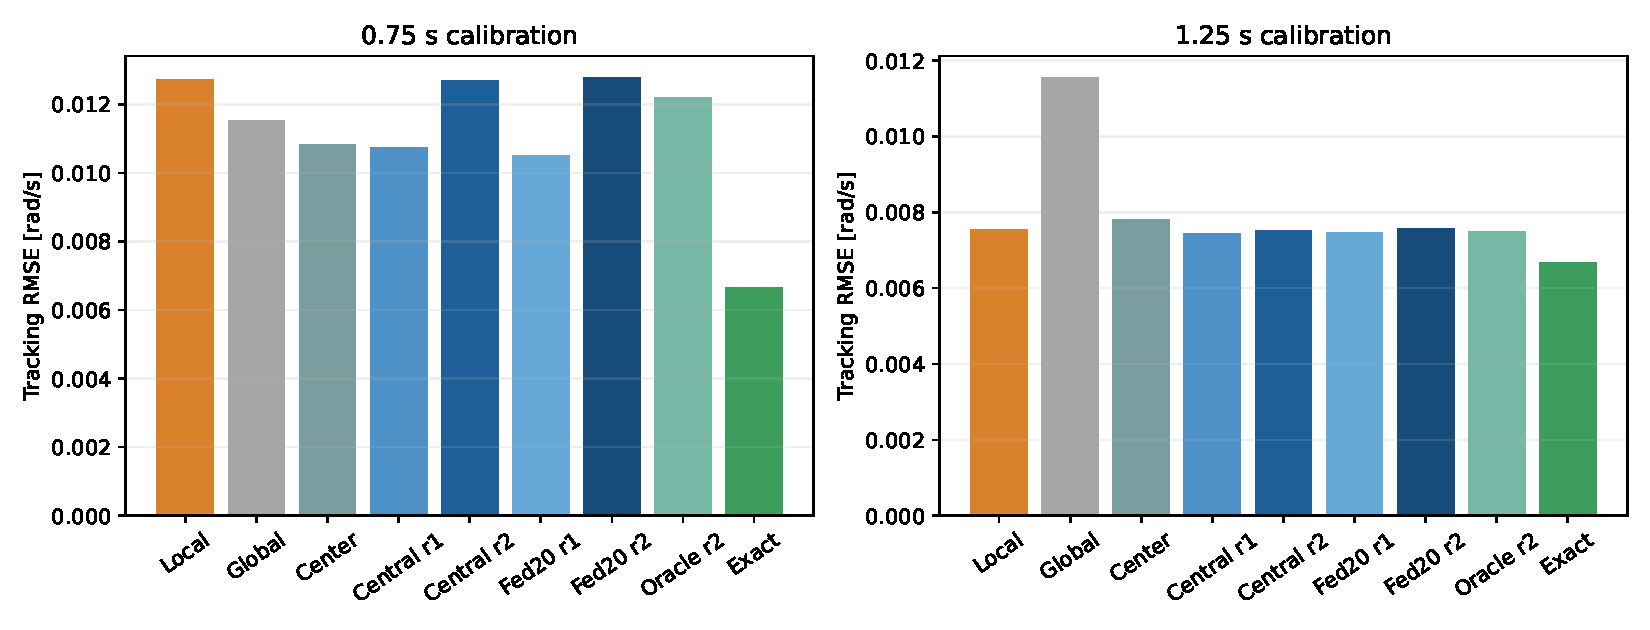
\includegraphics[width=\linewidth]{experiment_9m_unified_ablation.pdf}
\caption{Unified ablation of global sharing, latent group centers, and local
low-dimensional adaptation.}
\label{fig:ablation}
\end{figure}

\subsection{Participation rate versus fleet coverage}

Random rotating 20\% cohorts achieve 99.94\% cumulative client coverage and
retain the cold-start benefit even though their mean ARI is 0.917 rather than
one. Exact recovery of the synthetic generating families is therefore not
necessary for useful control.

The availability stress test reveals the relevant failure boundary. Rotating
family- or operating-point-biased cohorts and 50\% post-selection dropout still
improve the aggregate 0.75~s result over Local in the tested development fleets.
In contrast, repeatedly selecting one fixed narrow subset can collapse group
discovery; its variability increases sharply and one fleet becomes 34.43\%
worse than Local. Partial participation is thus safe neither by definition nor
by rate alone. Cumulative representation coverage is the operative condition.

\begin{figure}[t]
\centering
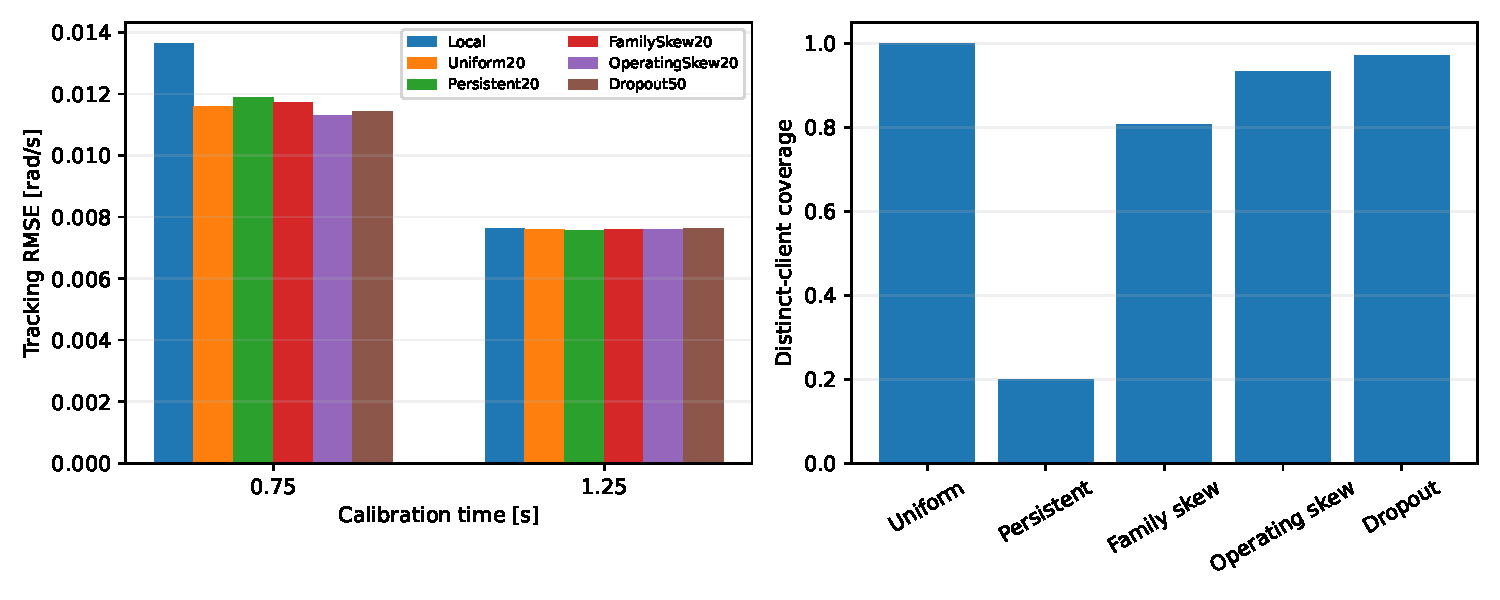
\includegraphics[width=\linewidth]{experiment_9l_nonrandom_participation.pdf}
\caption{Participation stress test. Rotating availability preserves broad
coverage; a persistent subset exposes the principal observed failure mode.}
\label{fig:participation}
\end{figure}

\subsection{Communication}

The unknown-order method fits every candidate $K=1,\ldots,6$; communication
must therefore include all candidates rather than only the selected model.
Table~\ref{tab:communication} reports corrected float32 payloads. Discovery is
a less frequent representation-learning operation, while the fixed-$K$ column
describes an update after the fleet has retained its selected order.

\begin{table}[t]
\centering
\caption{Mean confirmation-fleet payload. Upload/download are separated.}
\label{tab:communication}
\small
\begin{tabular}{lrr}
\toprule
Method & Discovery [MB] & Fixed-$K$ update [MB]\\
\midrule
Fed100 & 7.342 / 4.536 & 1.068 / 0.648\\
Fed50  & 3.691 / 2.268 & 0.546 / 0.324\\
Fed20  & 1.502 / 0.907 & 0.241 / 0.134\\
\bottomrule
\end{tabular}
\end{table}

\section{Discussion}
\label{sec:discussion}

\subsection{What federation contributes}

The benefit does not arise because distributed optimization improves an
already accurate local estimator. It arises because fleet-level observations
constrain an otherwise weak new-client problem. In statistical terms, the
learned group center supplies a heterogeneous empirical-Bayes prior, and the
rank-one coordinate defines a data-efficient client-specific head. In control
terms, the representation restricts early identification to parameter
variations that have been observed across the fleet and matter to the scheduled
gain map.

This interpretation explains both the positive and negative evidence. At
0.75~s, unconstrained three-parameter Local identification has excessive
variance, so group structure helps. At 1.25~s, the local record supports a
reliable displacement within the learned subspace. With still more excitation,
the independent local estimator can recover the full parameter vector and the
sharing advantage should vanish.

\subsection{Operational implications}

The results suggest that fleet-informed calibration should be deployed as a
transient prior rather than a permanent constraint. A practical system could
begin from the selected group center, enable the low-dimensional head once its
local information criterion is adequate, and finally release the full local
model after sufficient excitation. The participation audit further suggests a
server-side coverage monitor: accepting a nominal 20\% cohort is insufficient
if the same subpopulation repeatedly participates.

\subsection{Limitations}

The evidence is entirely simulation based. Vehicles are generated from three
physical populations, and the compact model contains only three ratios. The
unknown-order mechanism is nevertheless evaluated without access to those
labels; labels enter only the ARI audit and availability stress construction.
Validation on measured fleet data and a higher-dimensional LPV model remains
necessary to establish scalability and external validity.

The comparison is intentionally asymmetric: 180 fleet clients contribute more
total data than the new client. The claim is reduced new-client calibration,
not reduced total fleet data. Ten independent confirmation fleets provide
paired evidence but limited resolution of rare failures. The gain-weighted
basis approximates controller relevance locally and does not optimize nonlinear
closed-loop loss. Finally, raw-data locality is not equivalent to formal
privacy. The evaluated protocol neither implements cryptographic secure
aggregation nor differential privacy, and empirical feasibility is not a
formal nonlinear stability guarantee.

\section{Conclusion}
\label{sec:conclusion}

This paper formulated heterogeneous fleet learning as a cold-start transfer
problem for LPV controller calibration. An unknown-order federated mixture
learns reusable group structure from additive client statistics; a
controller-gain-aware low-rank backbone then provides a small local head for an
unseen vehicle. On nonlinear confirmation fleets, 20\% rotating participation
reduces tracking RMSE by 17.27\% at a 0.75~s calibration budget. The mechanism
analysis shows that learned group centers dominate under severe information
scarcity, while continuous personalization becomes useful as local information
increases. The benefit contracts to local parity and can fail when
participation lacks fleet coverage. Federated LPV identification should
therefore be understood as a coverage-dependent cold-start prior, not as a
universal substitute for local identification.

\begin{thebibliography}{9}

\bibitem{mcmahan2017fedavg}
H.~B. McMahan, E.~Moore, D.~Ramage, S.~Hampson, and B.~A. y Arcas,
``Communication-efficient learning of deep networks from decentralized data,''
in \emph{Proc. AISTATS}, 2017, pp.~1273--1282.

\bibitem{smith2017mocha}
V.~Smith, C.-K. Chiang, M.~Sanjabi, and A.~S. Talwalkar,
``Federated multi-task learning,'' in \emph{Advances in Neural Information
Processing Systems}, 2017.

\bibitem{fallah2020personalized}
A.~Fallah, A.~Mokhtari, and A.~Ozdaglar,
``Personalized federated learning with theoretical guarantees: A model-agnostic
meta-learning approach,'' in \emph{Advances in Neural Information Processing
Systems}, 2020.

\bibitem{toth2010lpv}
R.~T\'oth, \emph{Modeling and Identification of Linear Parameter-Varying
Systems}. Berlin, Germany: Springer, 2010.

\bibitem{weber2026ifac}
J.~Weber et al., ``Uncertainty-aware clustered federated identification for
controller design: Application to lateral dynamics and yaw-rate tracking,''
accepted for publication in \emph{Proc. IFAC World Congress}, 2026.

\end{thebibliography}

\end{document}
